\documentclass[../../thesis.tex]{subfiles}
%\graphicspath{{../../fig/}}

\begin{document}
\section{Computing Bigclam}
\label{sec:applying_bigclam}

Although the BIGCLAM algorithm output is the set of nodes belonging to a community, we are interested in the learned $\hat{F}$. Consequentially, we had to slightly modify the official BIGCLAM implementation provided at \href{https://github.com/snap-stanford/snap/tree/master/examples/bigclam}{Snap-stanford github page} in order to output the learned $\hat{F}$. 

To understand what the algorithm can provide for us, we run the BIGCLAM with our 3 Bitcoin data selected days as selected in the section \ref{sec:motifs_bitcoin}. Additionally, we induce our temporal network day samples into a static network by removing the time from the edges list. Thus, our day samples are now suitable as inputs for the BIGCLAM implementation. The result contains around 30 megabytes of static edges list for the day samples. We run BIGCLAM on those days on a cluster with Xeon E7 v3 36 cores and 128 GB of ram with the K=1 community. The algorithm took on average 20 minutes on each day sample to output its $\hat{F}$. 

After that, we run the Kolmogorov–Smirnov test \cite{massey1951kolmogorov} to discover which distribution fits best the $\hat{F}$. Testing on normal, log-normal, Pareto and Gamma distribution, the best fit was the log-normal distribution for all the selected days $\hat{F}$. We have done this procedure for days A, B, and C. We then plot the histogram of the result $\hat{F}$ and the result of the Kolmogorov–Smirnov test for the day A at figure \ref{fig:daymodel122_bigclam_f_hist}, for the day B at figure \ref{fig:daymodel165_bigclam_f_hist} and the day C at figure \ref{fig:daymodel210_bigclam_f_hist}. 

\begin{figure}[H]
\centering
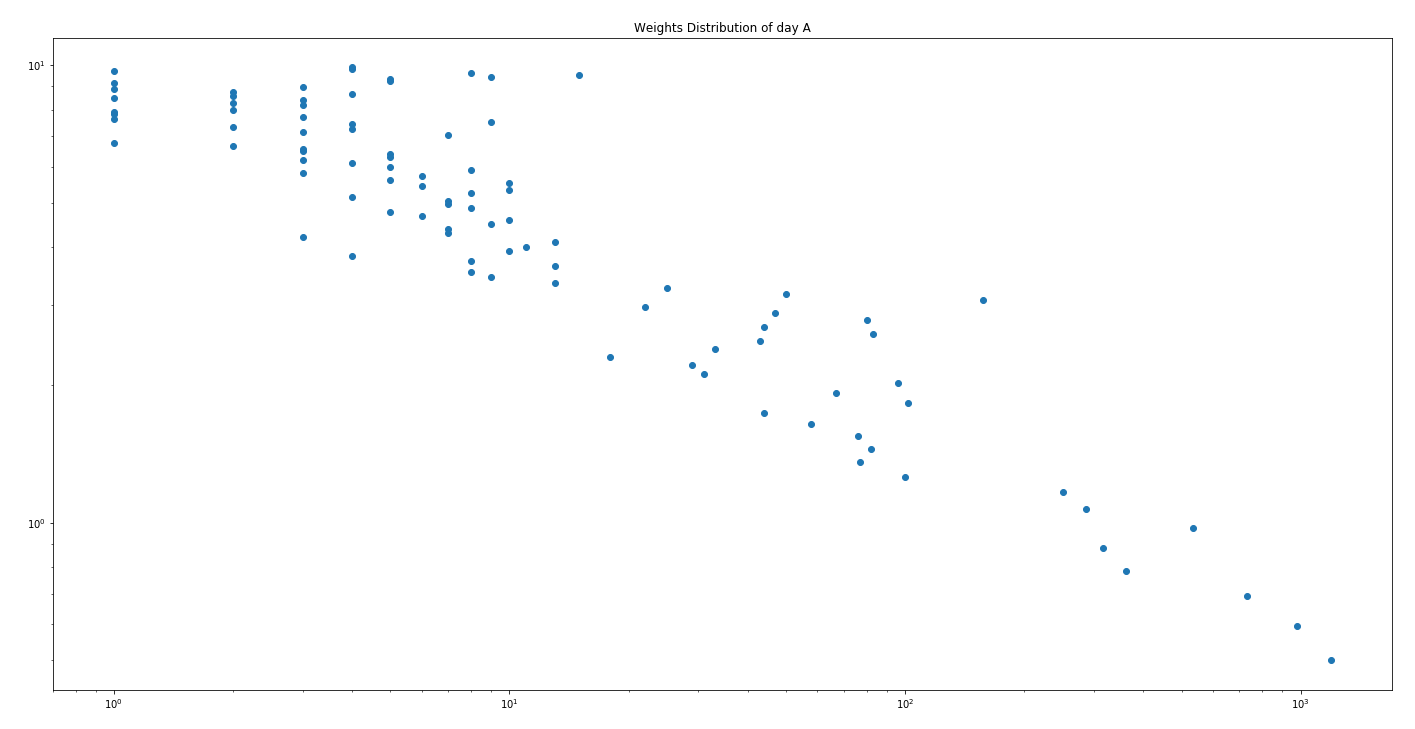
\includegraphics[width=\textwidth]{content/learning/img/daymodel122_bigclam_f_hist}
\caption{Histogram of the result $\hat{F}$ learned by the BIGCLAM algorithm for the \textbf{day A} $\hat{F}$. The result of the Kolmogorov–Smirnov test for the \textbf{day A} $\hat{F}$ has an error of $E=0.39$ for log-normal. $E=0.44$ for normal. $E=0.79$ for Pareto and $E=0.98$ for Gamma distribution. }
\label{fig:daymodel122_bigclam_f_hist}
\end{figure}

\begin{figure}[H]
\centering
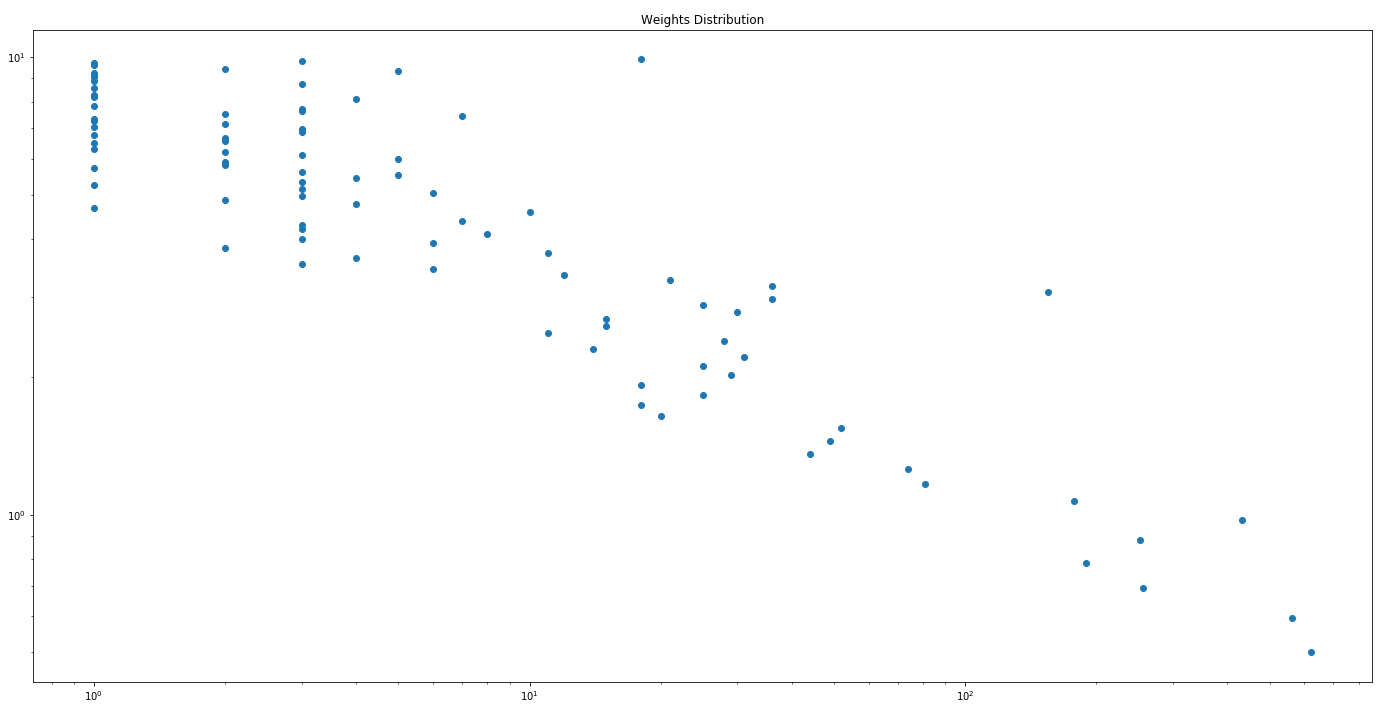
\includegraphics[width=\textwidth]{content/learning/img/daymodel165_bigclam_f_hist}
\caption{Histogram of the result $\hat{F}$ learned by the BIGCLAM algorithm for the \textbf{day B} $\hat{F}$. The result of the Kolmogorov–Smirnov test for the \textbf{day B} $\hat{F}$ has an error of $E=0.37$ for log-normal. $E=0.46$ for normal. $E=0.77$ for Pareto and $E=0.98$ for Gamma distribution. }
\label{fig:daymodel165_bigclam_f_hist}
\end{figure}

\begin{figure}[H]
\centering
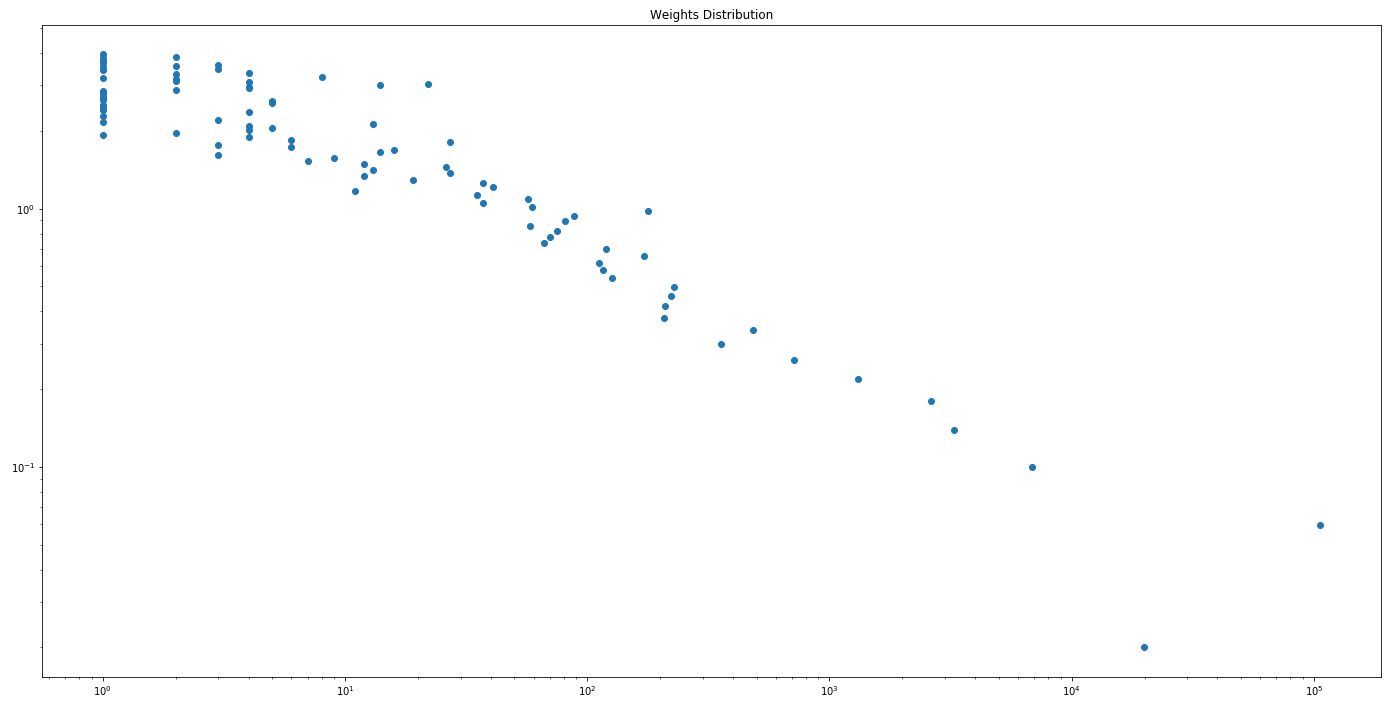
\includegraphics[width=\textwidth]{content/learning/img/daymodel210_bigclam_f_hist}
\caption{Histogram of the result $\hat{F}$ learned by the BIGCLAM algorithm for the \textbf{day C} $\hat{F}$. The result of the Kolmogorov–Smirnov test for the \textbf{day C} $\hat{F}$ has an error of $E=0.37$ for log-normal. $E=0.45$ for normal. $E=0.77$ for Pareto and $E=0.96$ for Gamma distribution. }
\label{fig:daymodel210_bigclam_f_hist}
\end{figure}


We now do the same above procedure as well, for the model A and Activity driven model produced in Section~\ref{sec:applying_proposed_activity_driven_model}. The result of $\hat{F}$ from model A memory size=5 can be seen in figure \ref{fig:memoryallBigclam151575059300_bigclam_f_hist} and for Activity driven model in figure \ref{fig:activitydrivenBigclam151574987200_bigclam_f_hist}. For the simulations, the BIGCLAM result in a log-norm distribution of $\hat{F}$ as well. However, for the model A memory size=5, the test results produced quite close errors for the normal $E=0.13231$, log-normal $E=0.13186$ and Gamma $E=0.13189$. Surprisingly, we can see that the memory model produced different BIGCLAM $\hat{F}$ comparing to the Active Driven model. 



\begin{figure}[H]
\centering
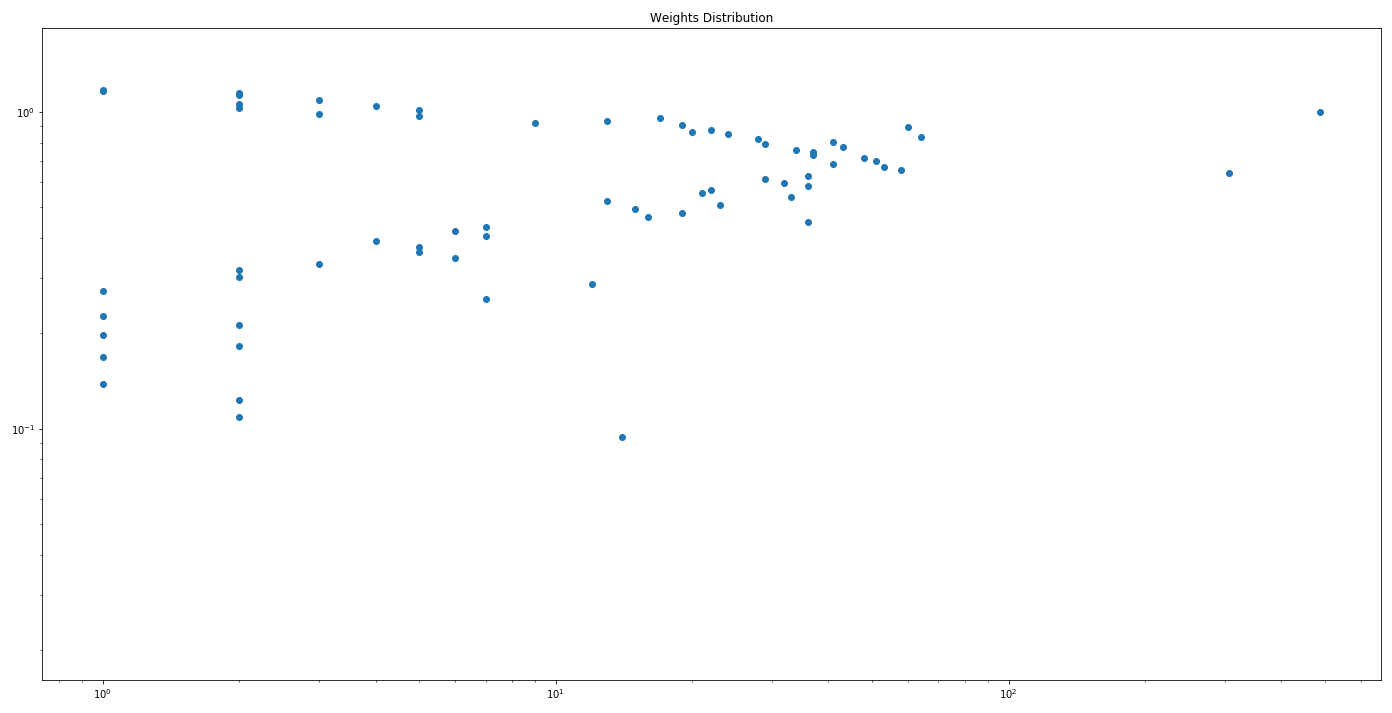
\includegraphics[width=\textwidth]{content/learning/img/memoryallBigclam151575059300_bigclam_f_hist}
\caption{Histogram of the result $\hat{F}$ learned by the BIGCLAM algorithm for the \textbf{model A memory size=5} $\hat{F}$. The result of the Kolmogorov–Smirnov test for the \textbf{model A memory size=5} $\hat{F}$ has an error of $E=0.13186$ for log-normal. $E=0.13231$ for normal. $E=0.38$ for Pareto and $E=0.13189$ for Gamma distribution. See that the results produced were quite close for log-normal and Gamma.}
\label{fig:memoryallBigclam151575059300_bigclam_f_hist}
\end{figure} 


\begin{figure}[H]
\centering
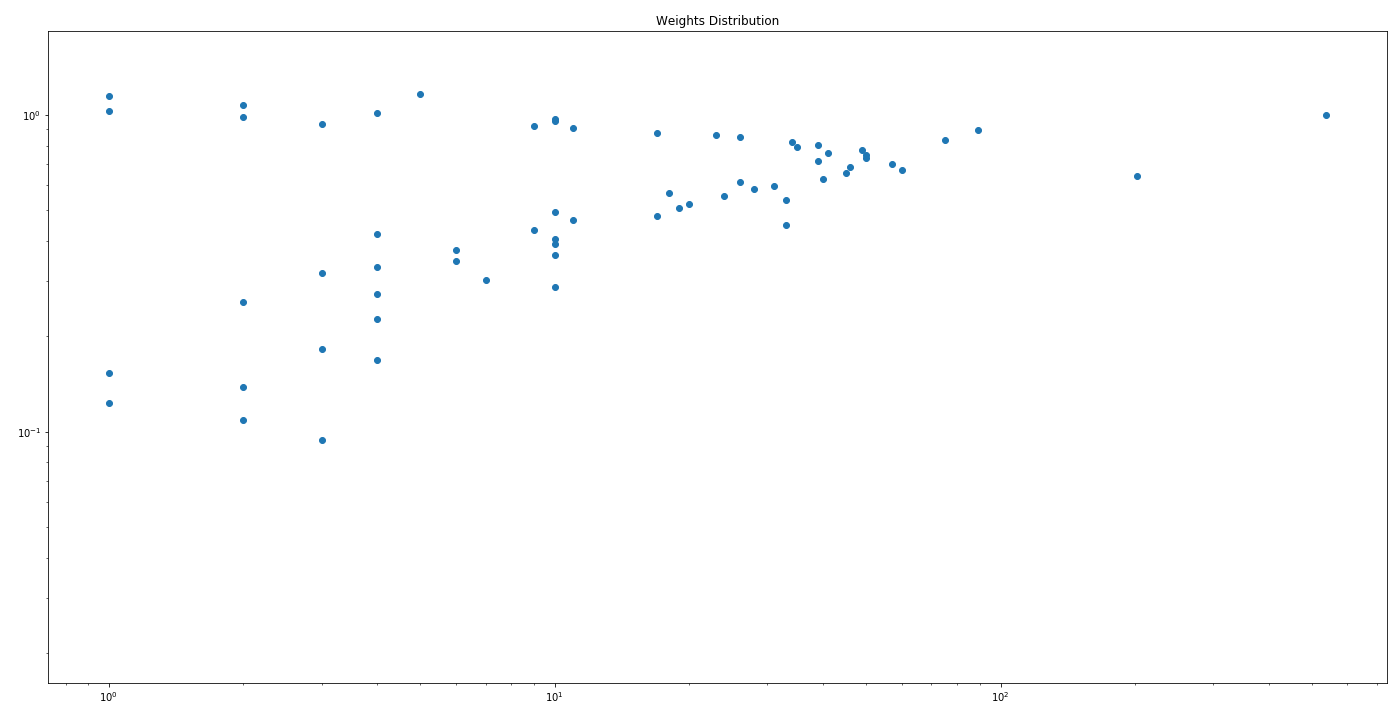
\includegraphics[width=\textwidth]{content/learning/img/activitydrivenBigclam151574987200_bigclam_f_hist}
\caption{Histogram of the result $\hat{F}$ learned by the BIGCLAM algorithm for the \textbf{Activity driven model} $\hat{F}$. The result of the Kolmogorov–Smirnov test for the \textbf{Activity driven model} $\hat{F}$ has an error of $E=0.17$ for log-normal. $E=0.30$ for normal. $E=0.38$ for Pareto and $E=0.48$ for Gamma distribution. }
\label{fig:activitydrivenBigclam151574987200_bigclam_f_hist}
\end{figure} 

We believe that the learned $\hat{F}$ from BIGCLAM can be used to derive the Activity potential distribution of the general model of Section~\ref{sec:activity_driven_model}, which could, in theory, be applied for predicting the Bitcoin temporal network. However, this is not a trivial task. Thus, we push this assignment for future work. 

\end{document}